%
\section{Example 2: BBOB}%
%
\xdef\bbobExamplePath{../../examples/bbob}%
%
\begin{frame}[t]%
\frametitle{BBOB}%
\begin{itemize}%
\item Since 2009, the \emph{Black-Box Optimization Benchmarking} (\bbob) workshops\scitep{\bbobReferences} regularly take place at GECCO (now also at CEC)%
\item<2-> Researchers can use the \emph{COmparing Continuous Optimisers} (\coco) framework to benchmark their \emph{numerical} optimization algorithms%
\item<3-> \coco/\bbob\ defines a set of 24 numerical optimization problems\uncover<4->{, which differ in features such as %
dimension\uncover<5->{, %
degree of separability\uncover<6->{, %
conditioning\uncover<7->{, %
etc.}}}}%
%
\item<8-> \coco\ can automatically run experiments, collect log files, and evaluate them%
\item<9-> The framework and the results of past {\bbob}s are available at \url{http://coco.gforge.inria.fr}%
\item<10-> \optimizationBenchmarking\ has an \alert{experimental} input driver for \coco\ data%
\item<11-> No need to specify \texttt{dimensions.xml} and \texttt{instances.xml}, as these are fixed and known for \coco/\bbob.% 
\end{itemize}%
%
\locate{3}{%
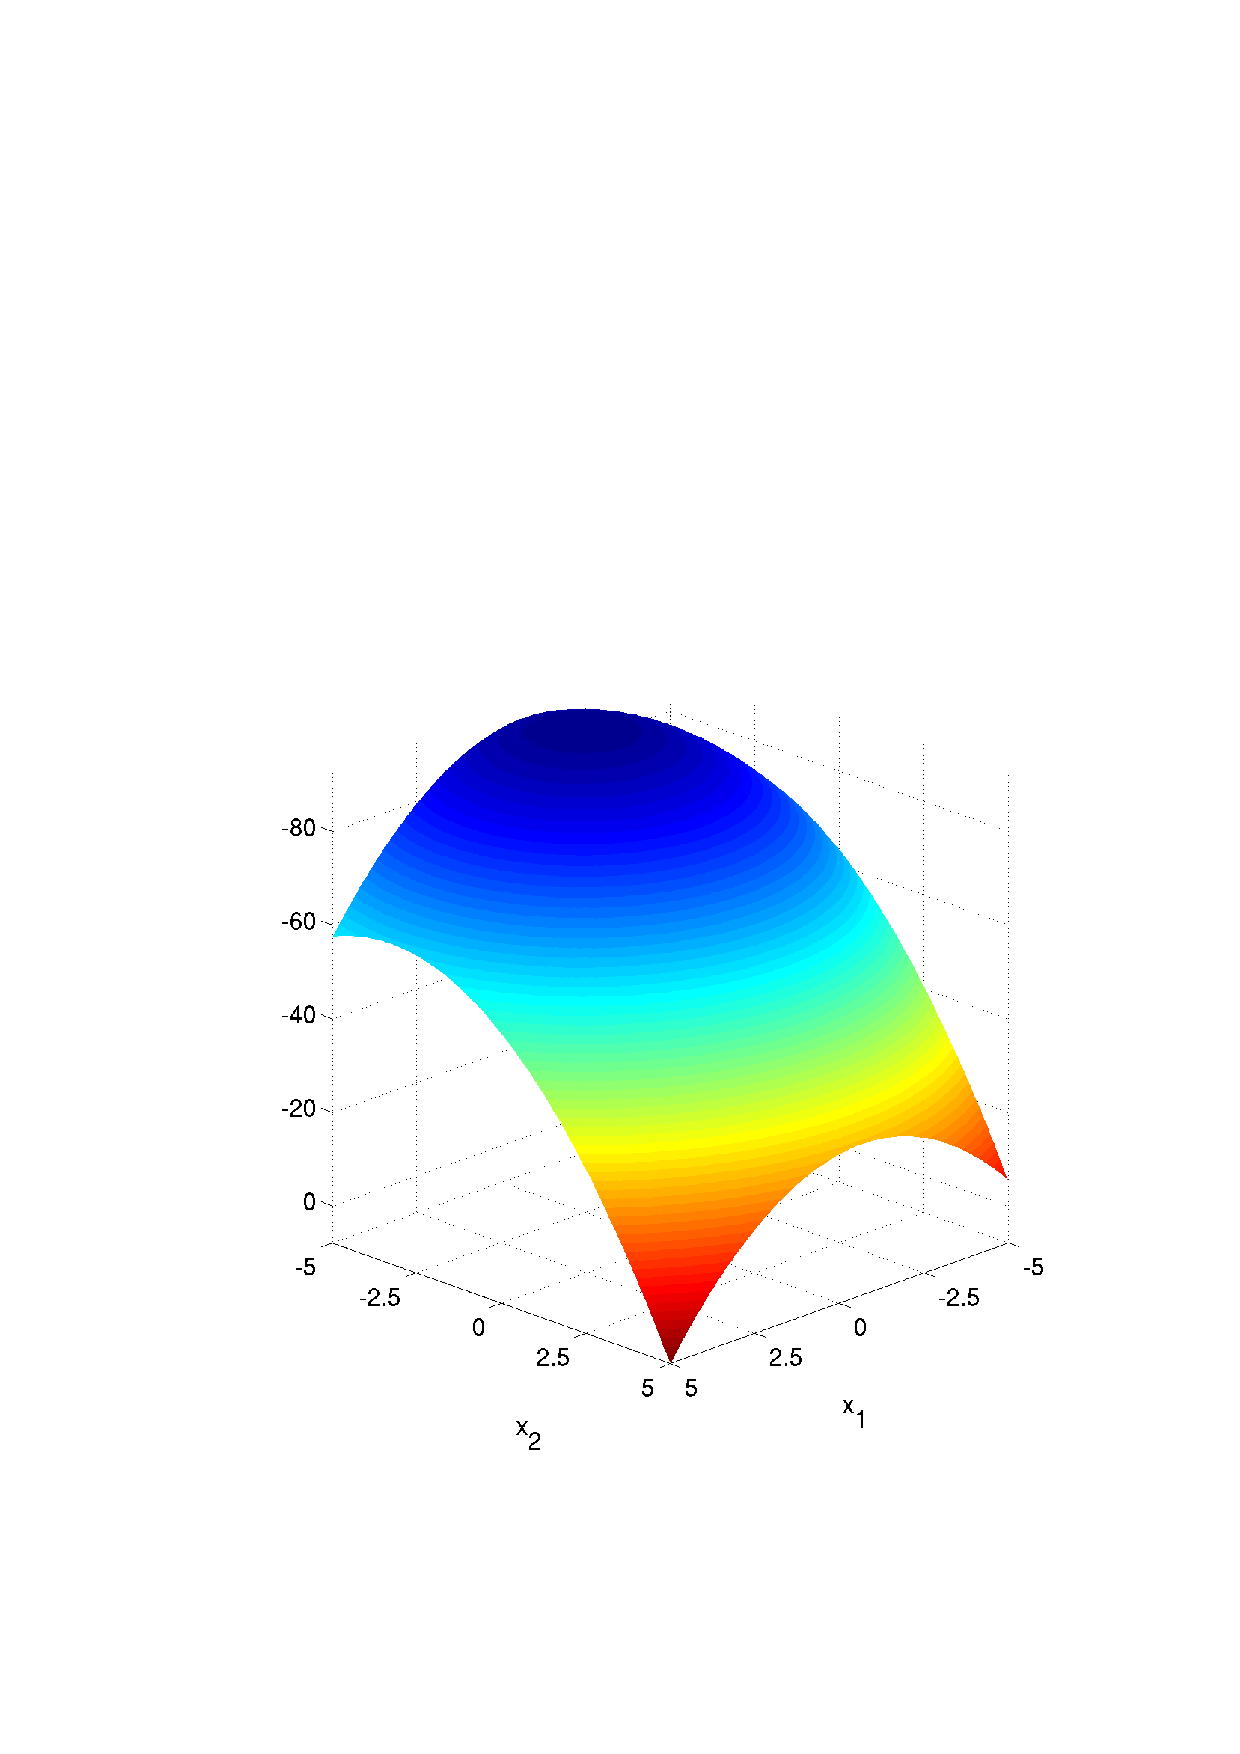
\includegraphics[page=1,width=0.108125\paperwidth]{\sharedPath/graphics/optimization/bbob/bbob_functions/bbob_functions}%%
}{0.015}{0.47125}%
\locate{3}{%
\includegraphics[page=2,width=0.108125\paperwidth]{\sharedPath/graphics/optimization/bbob/bbob_functions/bbob_functions}%%
}{0.138125}{0.47125}%
\locate{3}{%
\includegraphics[page=3,width=0.108125\paperwidth]{\sharedPath/graphics/optimization/bbob/bbob_functions/bbob_functions}%%
}{0.26125}{0.47125}%
\locate{3}{%
\includegraphics[page=4,width=0.108125\paperwidth]{\sharedPath/graphics/optimization/bbob/bbob_functions/bbob_functions}%%
}{0.384375}{0.47125}%
\locate{3}{%
\includegraphics[page=5,width=0.108125\paperwidth]{\sharedPath/graphics/optimization/bbob/bbob_functions/bbob_functions}%%
}{0.5075}{0.47125}%
\locate{3}{%
\includegraphics[page=6,width=0.108125\paperwidth]{\sharedPath/graphics/optimization/bbob/bbob_functions/bbob_functions}%%
}{0.630625}{0.47125}%
\locate{3}{%
\includegraphics[page=7,width=0.108125\paperwidth]{\sharedPath/graphics/optimization/bbob/bbob_functions/bbob_functions}%%
}{0.75375}{0.47125}%
\locate{3}{%
\includegraphics[page=8,width=0.108125\paperwidth]{\sharedPath/graphics/optimization/bbob/bbob_functions/bbob_functions}%%
}{0.876875}{0.47125}%
\locate{3}{%
\includegraphics[page=9,width=0.108125\paperwidth]{\sharedPath/graphics/optimization/bbob/bbob_functions/bbob_functions}%%
}{0.015}{0.619166666666667}%
\locate{3}{%
\includegraphics[page=10,width=0.108125\paperwidth]{\sharedPath/graphics/optimization/bbob/bbob_functions/bbob_functions}%%
}{0.138125}{0.619166666666667}%
\locate{3}{%
\includegraphics[page=11,width=0.108125\paperwidth]{\sharedPath/graphics/optimization/bbob/bbob_functions/bbob_functions}%%
}{0.26125}{0.619166666666667}%
\locate{3}{%
\includegraphics[page=12,width=0.108125\paperwidth]{\sharedPath/graphics/optimization/bbob/bbob_functions/bbob_functions}%%
}{0.384375}{0.619166666666667}%
\locate{3}{%
\includegraphics[page=13,width=0.108125\paperwidth]{\sharedPath/graphics/optimization/bbob/bbob_functions/bbob_functions}%%
}{0.5075}{0.619166666666667}%
\locate{3}{%
\includegraphics[page=14,width=0.108125\paperwidth]{\sharedPath/graphics/optimization/bbob/bbob_functions/bbob_functions}%%
}{0.630625}{0.619166666666667}%
\locate{3}{%
\includegraphics[page=15,width=0.108125\paperwidth]{\sharedPath/graphics/optimization/bbob/bbob_functions/bbob_functions}%%
}{0.75375}{0.619166666666667}%
\locate{3}{%
\includegraphics[page=16,width=0.108125\paperwidth]{\sharedPath/graphics/optimization/bbob/bbob_functions/bbob_functions}%%
}{0.876875}{0.619166666666667}%
\locate{3}{%
\includegraphics[page=17,width=0.108125\paperwidth]{\sharedPath/graphics/optimization/bbob/bbob_functions/bbob_functions}%%
}{0.015}{0.767083333333333}%
\locate{3}{%
\includegraphics[page=18,width=0.108125\paperwidth]{\sharedPath/graphics/optimization/bbob/bbob_functions/bbob_functions}%%
}{0.138125}{0.767083333333333}%
\locate{3}{%
\includegraphics[page=19,width=0.108125\paperwidth]{\sharedPath/graphics/optimization/bbob/bbob_functions/bbob_functions}%%
}{0.26125}{0.767083333333333}%
\locate{3}{%
\includegraphics[page=20,width=0.108125\paperwidth]{\sharedPath/graphics/optimization/bbob/bbob_functions/bbob_functions}%%
}{0.384375}{0.767083333333333}%
\locate{3}{%
\includegraphics[page=21,width=0.108125\paperwidth]{\sharedPath/graphics/optimization/bbob/bbob_functions/bbob_functions}%%
}{0.5075}{0.767083333333333}%
\locate{3}{%
\includegraphics[page=22,width=0.108125\paperwidth]{\sharedPath/graphics/optimization/bbob/bbob_functions/bbob_functions}%%
}{0.630625}{0.767083333333333}%
\locate{3}{%
\includegraphics[page=23,width=0.108125\paperwidth]{\sharedPath/graphics/optimization/bbob/bbob_functions/bbob_functions}%%
}{0.75375}{0.767083333333333}%
\locate{3}{%
\includegraphics[page=24,width=0.108125\paperwidth]{\sharedPath/graphics/optimization/bbob/bbob_functions/bbob_functions}%%
}{0.876875}{0.767083333333333}%
%
\locate{3}{%
\parbox{\paperwidth}{\centering%
\scriptsize{(figures taken from\scitep{FHRA2013RPBBOB2POTNF})}%
}}{0}{0.92}%
%
\locateWithCaption{4-7}{%
\pgfuseimage{bbob_features}%
}{%
The relative amounts of \bbob\ benchmark functions according to their features.%
}{0.0375}{0.54}{0.925}%
%
\end{frame}%
%
%
\begin{frame}[t,containsverbatim,fragile]
\frametitle{Quick Guide}%
%
\begin{itemize}%
\only<-2>{%
\item You can quickly download all example data and the Evaluator and run the example on your PC by executing the following code snippet.%
}%
\only<-2>{
\item<2-> System Requirements:%
\begin{itemize}%
\item Linux (for \texttt{make.sh}), Windows (for \texttt{make.bat}, tested: Win~8, should work also under Win~7)%
\item Java~1.7 (ideally a \texttt{JDK} under a \texttt{JRE} slower and higher memory consumption)%
\item \texttt{svn}%
\item optional: a \LaTeX\ installation, such as TeXLive (needed for generating pdf reports)%%
\end{itemize}%
}%
\only<3->{\item<3-> Enter (or create) a folder where you want to have everything, then execute this script via copy-paste to the terminal (it may need quite a while to run due to the downloads)}%
\only<6->{\item<5-> After the script, you will have%
\begin{itemize}%
\item a folder \texttt{results} with the log files which have been evaluated%
\item a folder \texttt{evaluation} with the configuration files and the \texttt{evaluation.xml} file defining what to do%
\item a filder \texttt{reports} with the generated reports%
\end{itemize}%
}%
%
\only<7->{%
\item<7-> But now, let's continue with the example\dots%
}%
\end{itemize}%
%
\only<4>{%
\begin{locateBox}{0.025}{0.29}
\begin{listingblock}[0.95\paperwidth]{Linux: script \texttt{make.sh} for downloading \& running the \bbob\ example.}
\centering
\begin{scaledBox}{!}{0.3\paperheight}
\parbox{1.8\paperwidth}{%
\lstinputlisting[language=bash,columns=fullflexible,mathescape=false,breaklines=true,breakatwhitespace=false,showstringspaces=false]{\bbobExamplePath/make.sh}
}%
\end{scaledBox}
\end{listingblock}
\end{locateBox}
}%
%
\only<5>{%
\begin{locateBox}{0.025}{0.29}
\begin{listingblock}[0.95\paperwidth]{Windows: script \texttt{make.sh} for downloading \& running the \bbob\ example.}
\centering
\begin{scaledBox}{!}{0.3\paperheight}
\parbox{2.2\paperwidth}{%
\lstinputlisting[language=command.com,columns=fullflexible,mathescape=false,breaklines=true,breakatwhitespace=false,showstringspaces=false]{\bbobExamplePath/make.bat}
}%
\end{scaledBox}
\end{listingblock}
\end{locateBox}
}%
%
\end{frame}
%
\begin{frame}%
\frametitle{Experiment}%
\begin{itemize}%
\item We select a set of experiments from the \bbob~2013 workshop for evaluation with the \optimizationBenchmarking\ Evaluator\uncover<2->{:%
\begin{enumerate}%
\item CMA-ES: \texttt{hutter2013\_CMAES.tar.gz}\scitep{HHLB2013AEOSMBOFEBF}%
\item<3-> IPOP-CMA-ES: \texttt{liao2013\_IPOP.tar.gz}\scitep{LS2013BTPSOICEOTNBT}%
\item<3-> IPOP-CMA-ES: \texttt{liao2013\_IPOP-500.tar.gz}\scitep{LS2013BTPSOICEOTNBT}%
\item<3-> IPOP-CMA-ES: \texttt{liao2013\_IPOP-tany.tar.gz}\scitep{LS2013TTIOPTOAVOICEWABMPSOTNBT}%
\item<3-> IPOP-CMA-ES: \texttt{liao2013\_IPOP-texp.tar.gz}\scitep{LS2013TTIOPTOAVOICEWABMPSOTNBT}%
\item<4-> Multi-Objectivization with NSGA-II\scitep{DAPM2000NSGA2}\texttt{tran2013\_P-DCN.tar.gz}\scitep{TBD2013MWNOTNBT}%
\item<5-> Differential Evolution (DE): \texttt{pal2013\_DE.tar.gz}\scitep{P2013BAHMLSLAOTBNT}%
\item<5-> Quasi-Newton Type Algorithm: \texttt{pal2013\_fmincon.tar.gz}\scitep{P2013COMGOAOTBNT}%
\item<5-> Nelder-Mead Simplex\scitep{NM1965ASMFFM}: \texttt{pal2013\_simplex.tar.gz}\scitep{P2013COMGOAOTBNT}%
\item<5-> Hybrid Multi-Level Single Linkage Algorithm (HMLSL): \texttt{pal2013\_HMLSL.tar.gz}\scitep{P2013BAHMLSLAOTBNT}%
\item<6-> Hill Climber: \texttt{holtschulte2013\_hill.tar.gz}\scitep{NM2013BCGAOTBNT}%
\item<6-> Generational GA: \texttt{holtschulte2013\_ga100.tar.gz}\scitep{NM2013BCGAOTBNT}%
\end{enumerate}%
}%
\item<7-> We can directly download them from \url{http://coco.lri.fr/BBOB2013/rawdata}\uncover<8->{\dots}%
\item<8-> {\dots}and unpack them into one common folder%
\end{itemize}%
\end{frame}%
%
\begin{frame}%
\frametitle{Evaluation}%
\begin{itemize}%
\item All we need to supply to the Evaluator is\uncover<2->{%
\begin{enumerate}%
\item the \texttt{evaluation.xml} file specifying what kind of information we want to obtain from the experimental data\uncover<3->{ and}%
\item<3-> the a configuration file (let's call it \texttt{configForIEEEtran.xml}) telling the Evaluator where everything is and what document driver or document class to use (guess which).%
\end{enumerate}%
}%
\item<4-> We now look at the interesting parts of the \texttt{evaluation.xml} file (the file in general has been discussed in the previous example)%
\end{itemize}%
\end{frame}% 
%
\begin{frame}[t,containsverbatim,fragile]
\frametitle{ECDF over Everything}%
\begin{itemize}%
\item Let's first plot the ECDF aggregated over all benchmark instances%
\only<-3>{%
\item<2-> We set the goal \inQuotes{error} to \numprint{1e-8}%
\item<3-> For the time measured in \measureFEs\ and log-scaled, we plot the fraction of runs achieving this goal%
}%
\end{itemize}%
%
\only<-3>{%
\begin{locateBox}{0.025}{0.425}
\begin{listingblock}[0.95\paperwidth]{Part~1 from file \texttt{evaluation.xml} for our \bbob\ example.}
\centering
\begin{scaledBox}{0.92\paperwidth}{!}
%\parbox{1.1\paperwidth}%
\end{scaledBox}
\end{listingblock}
\end{locateBox}
}%
%
\locate{4}{%
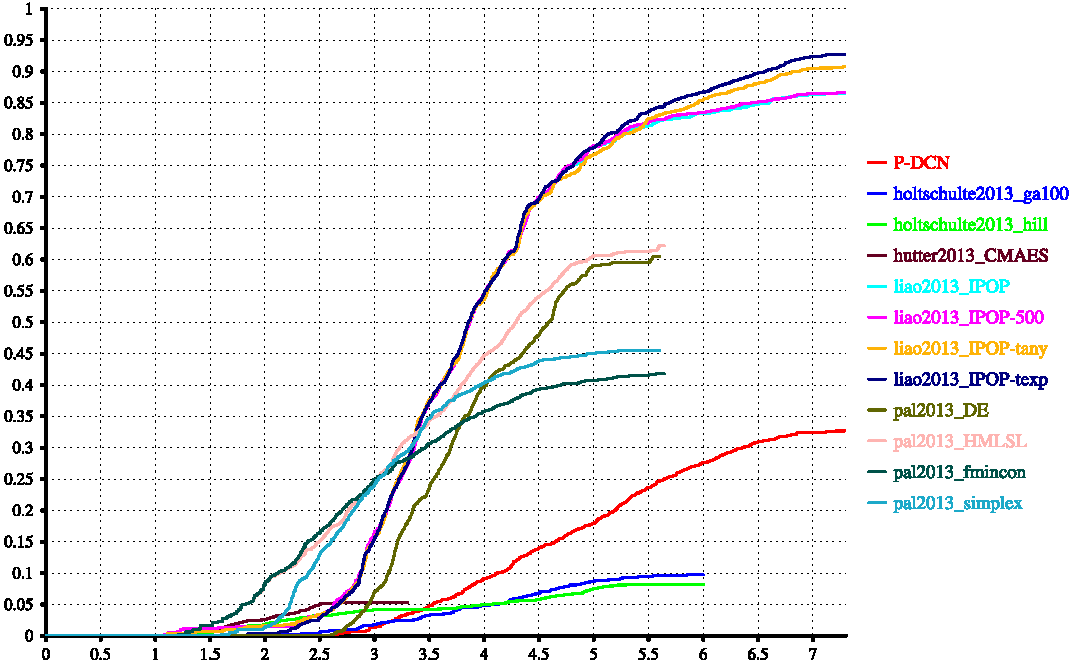
\includegraphics[width=0.9\paperwidth]{\sharedPath/graphics/optimization/bbob/bbob_example_evaluation/IEEEtran_ECDF_log_10_FEs_F_1_0E_8}%
}{0.05}{0.2}%
%
%
\locate{5-}{%
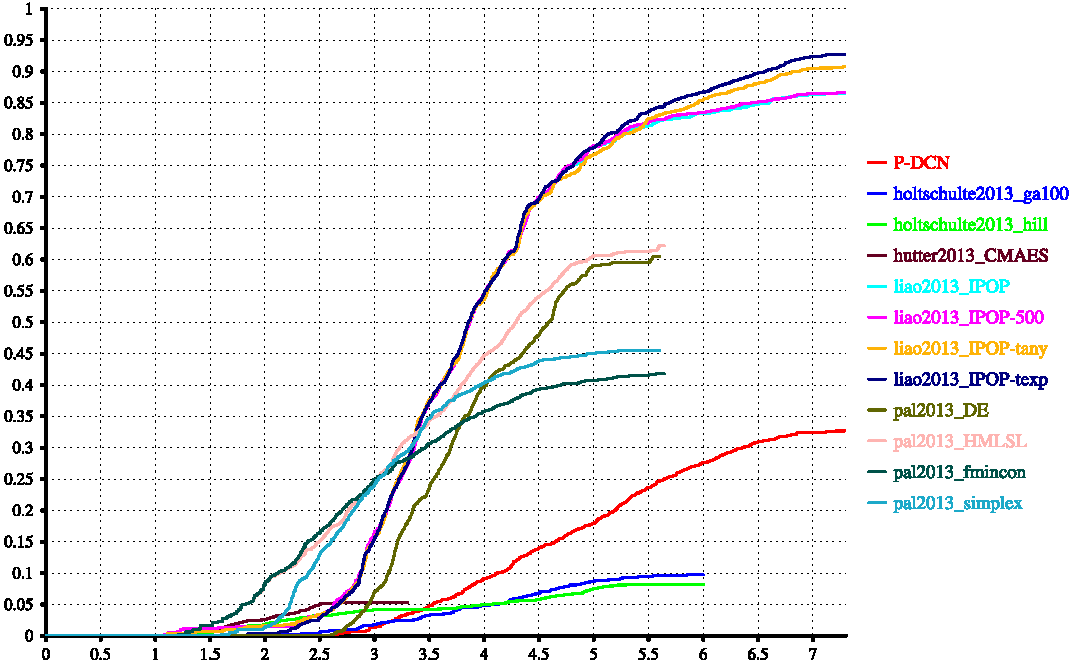
\includegraphics[width=0.5\paperwidth]{\sharedPath/graphics/optimization/bbob/bbob_example_evaluation/IEEEtran_ECDF_log_10_FEs_F_1_0E_8}%
}{0.025}{0.333}%
%
\locate{5-}{\parbox{0.45\paperwidth}{\footnotesize%
\begin{itemize}%
\item \footnotesize{It seems that \texttt{IPOP-texp} can reach $\measureObjectiveValue\leq\numprint{1e-8}$ on more instances than the other tested algorithms}%
\item<6-> \footnotesize{The different \texttt{IPOP} variants in general reach this value more often than the other algorithms}%
\item<7-> \footnotesize{\texttt{pal2013\_fmincon} and \texttt{pal2013\_HMLSL} both solve more problems during approximately the first \numprint{2500}~\measureFEs, i.e., are initially faster}%
\item<8-> \footnotesize{The Hill Climber and GA (\texttt{holtshulte}) solve the least problems in the comparison}%
\end{itemize}%
}}{0.525}{0.215}%
%
\end{frame}
%
%
%
\begin{frame}[t,containsverbatim,fragile]
\frametitle{ECDF by Dimension}%
%
\begin{itemize}%
\only<-4>{%
\item Let's now plot the ECDF aggregated over each distinct value of the benchmark feature \emph{dimension}%
\only<-3>{%
\item<2-> The goal \inQuotes{error} to achieve is again \numprint{1e-8}\uncover<3->{ and}%
\item<3-> also use the (only) time measured in \measureFEs, log-scaled.%
}}%
%
\only<5>{%
\item<5> We find that for larger dimension, fewer problems can be solved%
}%
\only<6>{%
\item<6> While the overall performance of \texttt{pal2013\_fmincon} and \texttt{pal2013\_simplex} look similar when considering \emph{all} problems, we find that the simplex algorithm is very heavily influenced by the dimension%  
}%
%
\only<7>{%
\item<7> Similarly, the performance of DE breaks down when the dimension increases% 
}%
%
\only<8->{%
\item<8> The performance of the IPOP algorithm family, on the other hand, degenerates gracefully with rising dimension%
}%
\end{itemize}%
%
\only<-3>{%
\begin{locateBox}{0.025}{0.425}
\begin{listingblock}[0.95\paperwidth]{Part~2 from file \texttt{evaluation.xml} for our \bbob\ example.}
\centering
\begin{scaledBox}{0.92\paperwidth}{!}
\lstinputlisting[language=XML,breaklines=true,breakatwhitespace=false,showstringspaces=false,linerange={22-29}]{\bbobExamplePath/evaluation/evaluation.xml}
\end{scaledBox}
\end{listingblock}
\end{locateBox}
}%
%
\locate{4-}{%
\parbox{0.313333333333333\paperwidth}{\centering%
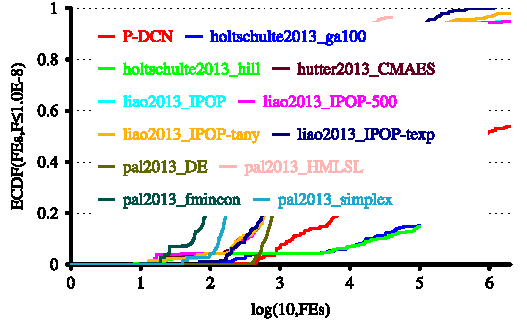
\includegraphics[width=0.313333333333333\paperwidth]{\sharedPath/graphics/optimization/bbob/bbob_example_evaluation/ECDF_log_10_FEs_F_1_0E_8_distinct_dim/IEEEtran_ECDF_log_10_FEs_F_1_0E_8_distinct_dim_legend.pdf}%%
\\%
\scriptsize{legend}%
}}{0.015}{0.33}%
%
\locate{4-}{%
\parbox{0.313333333333333\paperwidth}{\centering%
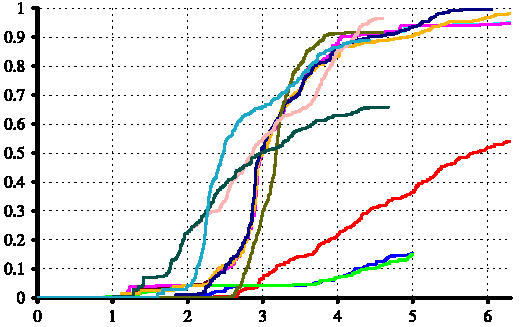
\includegraphics[width=0.313333333333333\paperwidth]{\sharedPath/graphics/optimization/bbob/bbob_example_evaluation/ECDF_log_10_FEs_F_1_0E_8_distinct_dim/IEEEtran_ECDF_log_10_FEs_F_1_0E_8_distinct_dim_2.pdf}%%
\\%
\scriptsize{$\texttt{dim}=2$}%
}}{0.343333333333333}{0.33}%
%
\locate{4-}{%
\parbox{0.313333333333333\paperwidth}{\centering%
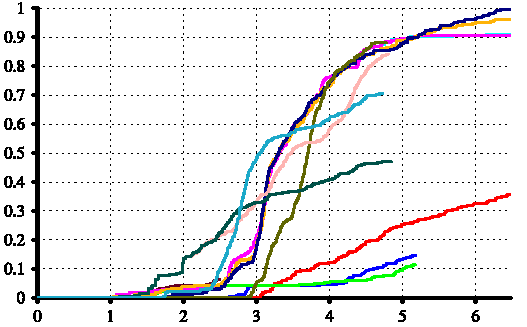
\includegraphics[width=0.313333333333333\paperwidth]{\sharedPath/graphics/optimization/bbob/bbob_example_evaluation/ECDF_log_10_FEs_F_1_0E_8_distinct_dim/IEEEtran_ECDF_log_10_FEs_F_1_0E_8_distinct_dim_3.pdf}%%
\\%
\scriptsize{$\texttt{dim}=4$}%
}}{0.671666666666667}{0.33}%
%
\locate{4-}{%
\parbox{0.313333333333333\paperwidth}{\centering%
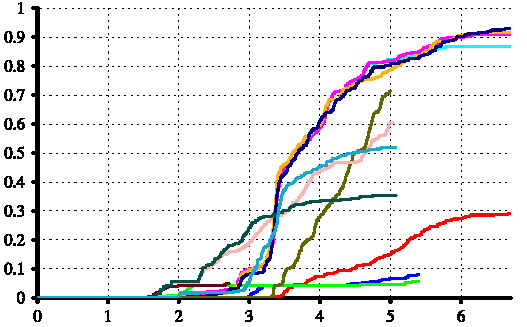
\includegraphics[width=0.313333333333333\paperwidth]{\sharedPath/graphics/optimization/bbob/bbob_example_evaluation/ECDF_log_10_FEs_F_1_0E_8_distinct_dim/IEEEtran_ECDF_log_10_FEs_F_1_0E_8_distinct_dim_5.pdf}%%
\\%
\scriptsize{$\texttt{dim}=5$}%
}}{0.015}{0.6444}%
%
\locate{4-}{%
\parbox{0.313333333333333\paperwidth}{\centering%
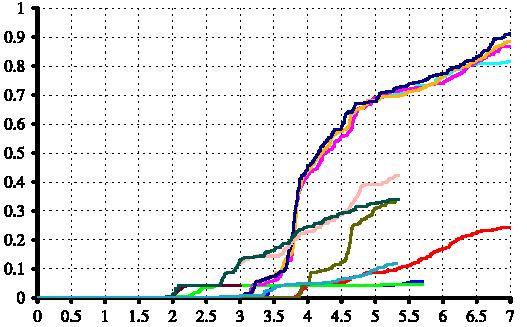
\includegraphics[width=0.313333333333333\paperwidth]{\sharedPath/graphics/optimization/bbob/bbob_example_evaluation/ECDF_log_10_FEs_F_1_0E_8_distinct_dim/IEEEtran_ECDF_log_10_FEs_F_1_0E_8_distinct_dim_10.pdf}%%
\\%
\scriptsize{$\texttt{dim}=10$}%
}}{0.343333333333333}{0.6444}%
%
\locate{4-}{%
\parbox{0.313333333333333\paperwidth}{\centering%
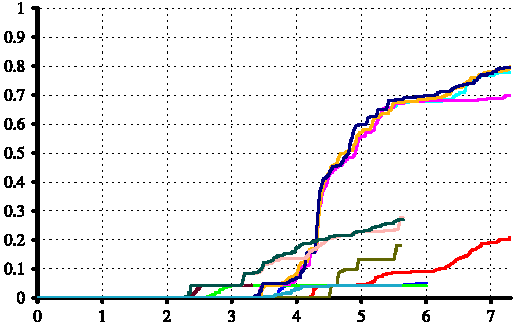
\includegraphics[width=0.313333333333333\paperwidth]{\sharedPath/graphics/optimization/bbob/bbob_example_evaluation/ECDF_log_10_FEs_F_1_0E_8_distinct_dim/IEEEtran_ECDF_log_10_FEs_F_1_0E_8_distinct_dim_20.pdf}%%
\\%
\scriptsize{$\texttt{dim}=20$}%
}}{0.671666666666667}{0.6444}%
%
%
\end{frame}
%
%
%
%
\begin{frame}[t,containsverbatim,fragile]
\frametitle{ECDF by Condition Number}%
%
\begin{itemize}%
\only<-4>{%
\item Let's now plot the ECDF aggregated over the benchmark instances with the same value of feature \emph{condition number}%
\only<-3>{%
\item<2-> \emph{\inQuotes{the condition number corresponds to the square root of the ratio between the largest axis of the ellipsoid and the shortest axis}}\scitep{FHRA2013RPBBOB2POTNF}% 
\item<3-> As goal \inQuotes{error} to achieve, this time we pick \numprint{1e-5}%
}}%
%
\only<5>{%
\item<5> The influence of the condition number on problem hardness does not seem to obvious at first glance%
}%
%
\only<6>{%
\item<6> Some algorithms perform bad on some mediocre condition numbers while performing better on smaller and larger ones (e.g., \texttt{P-DCN} on $\texttt{cond}=\numprint{1000}$)%
}%
%
\only<7>{%
\item<7> For some problems, there doesn't seem to be a direct relationship between conditioning and performance (e.g., DE)% 
}%
%
\only<8-10>{%
\item<8-10> Possible reason\only<9>{s}: The problems in the benchmark belonging to a certain condition number may have various other features making them hard or easy\only<9->{\only<9>{ and}\only<10->{,} %
the number of problems per condition number differs largely\only<10->{, and %
the goal value \numprint{1e-5} may be too easy to achieve, leading to a large variance in the results%
}}}%
%
\end{itemize}%
%
\only<-3>{%
\begin{locateBox}{0.025}{0.425}
\begin{listingblock}[0.95\paperwidth]{Part~3 from file \texttt{evaluation.xml} for our \bbob\ example.}
\centering
\begin{scaledBox}{0.92\paperwidth}{!}
\lstinputlisting[language=XML,breaklines=true,breakatwhitespace=false,showstringspaces=false,linerange={31-38}]{\bbobExamplePath/evaluation/evaluation.xml}
\end{scaledBox}
\end{listingblock}
\end{locateBox}
}%
%
\locate{4-8}{\parbox{0.23125\paperwidth}{\centering%%
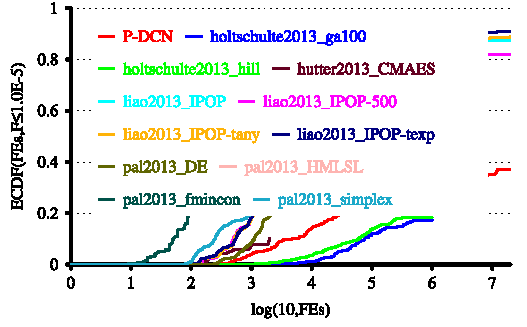
\includegraphics[width=0.23125\paperwidth]{\sharedPath/graphics/optimization/bbob/bbob_example_evaluation/ECDF_log_10_FEs_F_1_0E_5_distinct_cond/IEEEtran_ECDF_log_10_FEs_F_1_0E_5_distinct_cond_legend.pdf}%%
\\%
\scriptsize{legend}%
}}{0.015}{0.35}%
%
\locate{4-8}{\parbox{0.23125\paperwidth}{\centering%%
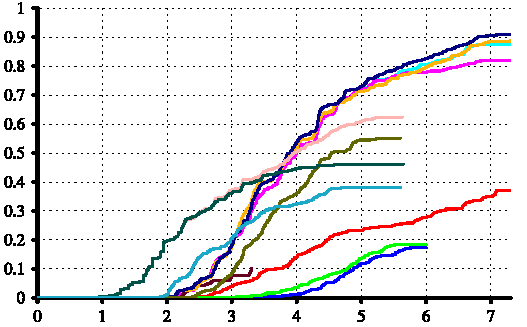
\includegraphics[width=0.23125\paperwidth]{\sharedPath/graphics/optimization/bbob/bbob_example_evaluation/ECDF_log_10_FEs_F_1_0E_5_distinct_cond/IEEEtran_ECDF_log_10_FEs_F_1_0E_5_distinct_cond_1.pdf}%%
\\%
\scriptsize{$\texttt{cond}=\numprint{1}$}%
}}{0.26125}{0.35}%
%
\locate{4-8}{\parbox{0.23125\paperwidth}{\centering%%
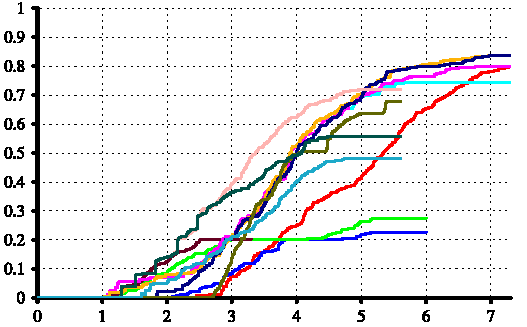
\includegraphics[width=0.23125\paperwidth]{\sharedPath/graphics/optimization/bbob/bbob_example_evaluation/ECDF_log_10_FEs_F_1_0E_5_distinct_cond/IEEEtran_ECDF_log_10_FEs_F_1_0E_5_distinct_cond_10.pdf}%%
\\%
\scriptsize{$\texttt{cond}=\numprint{10}$}%
}}{0.5075}{0.35}%
%
\locate{4-8}{\parbox{0.23125\paperwidth}{\centering%%
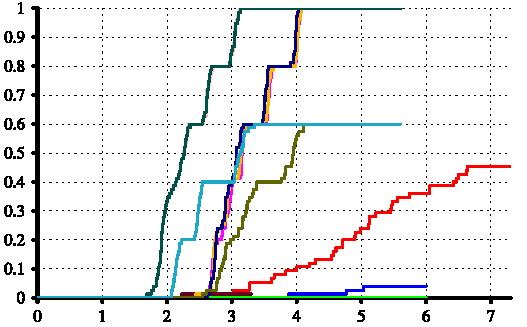
\includegraphics[width=0.23125\paperwidth]{\sharedPath/graphics/optimization/bbob/bbob_example_evaluation/ECDF_log_10_FEs_F_1_0E_5_distinct_cond/IEEEtran_ECDF_log_10_FEs_F_1_0E_5_distinct_cond_25.pdf}%%
\\%
\scriptsize{$\texttt{cond}=\numprint{25}$}%
}}{0.75375}{0.35}%
%
\locate{4-8}{\parbox{0.23125\paperwidth}{\centering%%
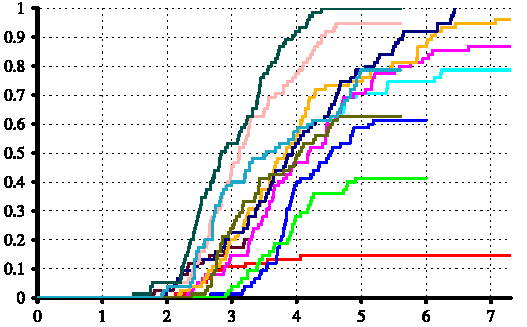
\includegraphics[width=0.23125\paperwidth]{\sharedPath/graphics/optimization/bbob/bbob_example_evaluation/ECDF_log_10_FEs_F_1_0E_5_distinct_cond/IEEEtran_ECDF_log_10_FEs_F_1_0E_5_distinct_cond_30.pdf}%%
\\%
\scriptsize{$\texttt{cond}=\numprint{30}$}%
}}{0.015}{0.6325}%
%
\locate{4-8}{\parbox{0.23125\paperwidth}{\centering%%
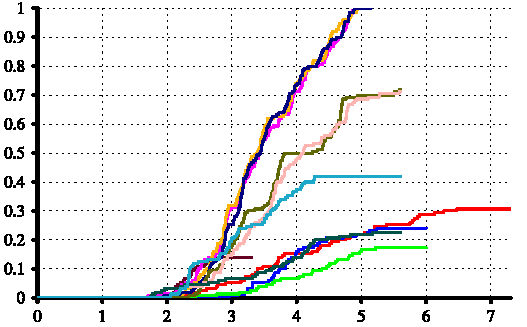
\includegraphics[width=0.23125\paperwidth]{\sharedPath/graphics/optimization/bbob/bbob_example_evaluation/ECDF_log_10_FEs_F_1_0E_5_distinct_cond/IEEEtran_ECDF_log_10_FEs_F_1_0E_5_distinct_cond_100.pdf}%%
\\%
\scriptsize{$\texttt{cond}=\numprint{100}$}%
}}{0.26125}{0.6325}%
%
\locate{4-8}{\parbox{0.23125\paperwidth}{\centering%%
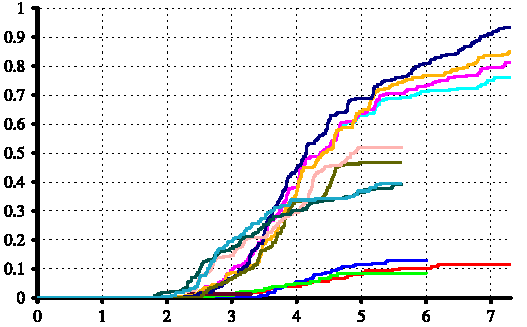
\includegraphics[width=0.23125\paperwidth]{\sharedPath/graphics/optimization/bbob/bbob_example_evaluation/ECDF_log_10_FEs_F_1_0E_5_distinct_cond/IEEEtran_ECDF_log_10_FEs_F_1_0E_5_distinct_cond_1000.pdf}%%
\\%
\scriptsize{$\texttt{cond}=\numprint{1000}$}%
}}{0.5075}{0.6325}%
%
\locate{4-8}{\parbox{0.23125\paperwidth}{\centering%%
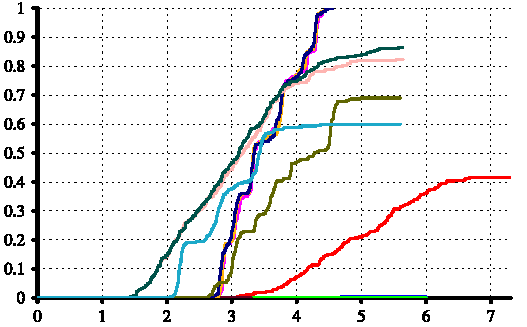
\includegraphics[width=0.23125\paperwidth]{\sharedPath/graphics/optimization/bbob/bbob_example_evaluation/ECDF_log_10_FEs_F_1_0E_5_distinct_cond/IEEEtran_ECDF_log_10_FEs_F_1_0E_5_distinct_cond_1000000.pdf}%%
\\%
\scriptsize{$\texttt{cond}=\numprint{1000000}$}%
}}{0.75375}{0.6325}%
%
\locateWithCaption{9}{%
\pgfuseimage{bbob_features}%
}{%
The relative amounts of \bbob\ benchmark functions according to their features.\\%
(This diagram has also been created with \optimizationBenchmarking.)%
}{0.0375}{0.52}{0.925}%
%
%
\begin{locateBox}[9]{0}{0}
\begin{pgfpicture}%
\pgfpathrectangle{\pgfpoint{0pt}{0pt}}{\pgfpoint{\paperwidth}{\paperheight}}%
\pgfusepath{use as bounding box,clip}%
\pgfsetcolor{alertviolet}%
\pgfsetlinewidth{2pt}%
\pgfpathrectangle{\pgfpoint{0.755\paperwidth}{0.19\paperheight}}{\pgfpoint{0.22\paperwidth}{0.3333\paperheight}}%
\pgfusepath{stroke}%
\end{pgfpicture}%
\end{locateBox}%
%
%
\end{frame}
%
%
%
%
%
%
%
\begin{frame}[t,containsverbatim,fragile]
\frametitle{Progress by Separability}%
%
\begin{itemize}%
\only<-4>{%
\item Finally, let's see how the algorithms progress on problems of different degrees of separability%
\only<-3>{%
\item<2-> The x-axis be again the log-scaled \measureFEs\ divided by the square of the benchmark instance dimension\footnote<2>{%
Yes, the square. Because \emph{why not}. You can do arbitrary mathematical expressions (as long as the preserve the order of the values)%
}\uncover<3->{ and}%
\item<3-> on the y-axis, we plot the median of the log-scaled objective value \measureObjectiveValue%
}}%
%
\only<5>{%
\item<5> We find that \texttt{pal2013\_fmincon} and \texttt{pal2013\_HMLSL} are quite good in solving fully and partially separable problems but both (and especially \texttt{pal2013\_fmincon}) perform worse on non-separable problems%
}%
%
\only<6>{%
\item<6> Here seems to be the strength of the \texttt{IPOP} family of algorithms%
}%
%
\only<7>{%
\item<7> Generally, a decrease in separability, i.e., stronger \inQuotes{variable interactions}\scitep{CWYT2010LSGOUCCWVIL}, makes optimization problems harder for numerical optimization algorithms, which either need longer to or cease to achieve high-quality solutions%
}%
%
\end{itemize}%
%
\only<-3>{%
\begin{locateBox}{0.025}{0.425}
\begin{listingblock}[0.95\paperwidth]{Part~4 from file \texttt{evaluation.xml} for our \bbob\ example.}
\centering
\begin{scaledBox}{0.92\paperwidth}{!}
\lstinputlisting[language=XML,breaklines=true,breakatwhitespace=false,showstringspaces=false,linerange={40-47}]{\bbobExamplePath/evaluation/evaluation.xml}
\end{scaledBox}
\end{listingblock}
\end{locateBox}
}%
%
%
\locate{4-}{%
\parbox{0.4775\paperwidth}{\centering%
\rotatebox{90}{\mbox{\strut\scriptsize{\strut~~~~~~~~~~~~legend}}}%
~%
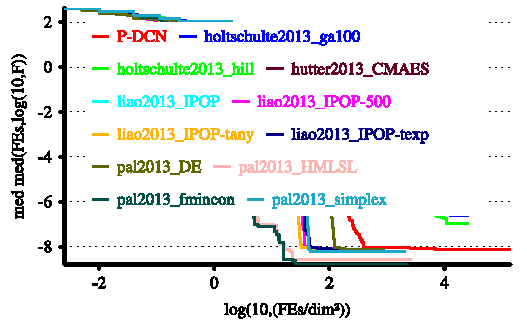
\includegraphics[width=0.33\paperwidth]{\sharedPath/graphics/optimization/bbob/bbob_example_evaluation/med_med_log_10_FEs_dim2_log_10_F_distinct_sep/IEEEtran_med_med_log_10_FEs_dim2_log_10_F_distinct_sep_legend.pdf}%%
}}{0.015}{0.35}%
%
\locate{4-}{%
\parbox{0.4775\paperwidth}{\centering%
\rotatebox{90}{\mbox{\strut\scriptsize{\strut~~~~~~fully separable}}}%
~%
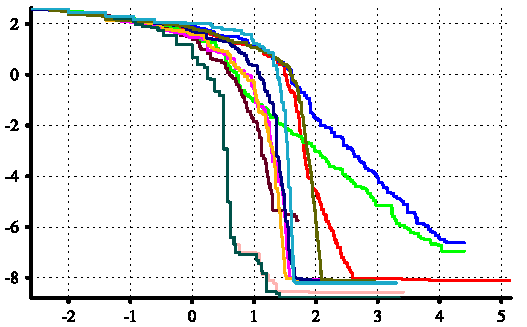
\includegraphics[width=0.33\paperwidth]{\sharedPath/graphics/optimization/bbob/bbob_example_evaluation/med_med_log_10_FEs_dim2_log_10_F_distinct_sep/IEEEtran_med_med_log_10_FEs_dim2_log_10_F_distinct_sep_fully.pdf}%%
}}{0.5075}{0.35}%
%
\locate{4-}{%
\parbox{0.4775\paperwidth}{\centering%
\rotatebox{90}{\mbox{\strut\scriptsize{\strut~~~partially separable}}}%
~%
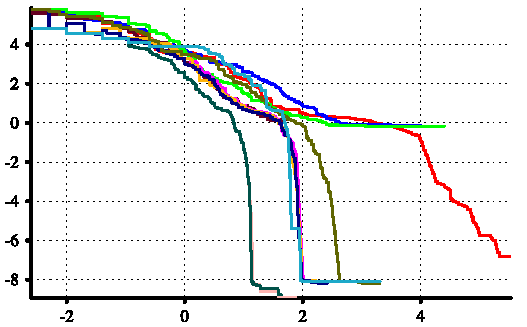
\includegraphics[width=0.33\paperwidth]{\sharedPath/graphics/optimization/bbob/bbob_example_evaluation/med_med_log_10_FEs_dim2_log_10_F_distinct_sep/IEEEtran_med_med_log_10_FEs_dim2_log_10_F_distinct_sep_partially.pdf}%%
}}{0.015}{0.6525}%
%
\locate{4-}{%
\parbox{0.4775\paperwidth}{\centering%
\rotatebox{90}{\mbox{\strut\scriptsize{\strut~~~~~~non-separable}}}%
~%
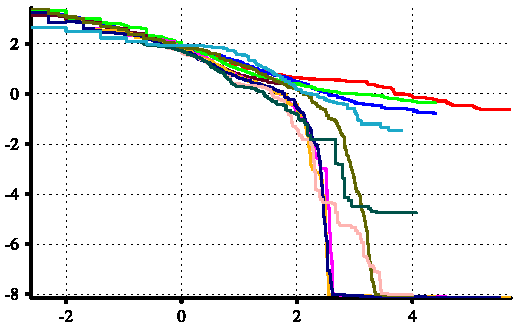
\includegraphics[width=0.33\paperwidth]{\sharedPath/graphics/optimization/bbob/bbob_example_evaluation/med_med_log_10_FEs_dim2_log_10_F_distinct_sep/IEEEtran_med_med_log_10_FEs_dim2_log_10_F_distinct_sep_none.pdf}%%
}}{0.5075}{0.6525}%"
%
%
%
\end{frame}
%
%
\begin{frame}%
\frametitle{Example Summary}%
\parbox{0.525\paperwidth}{%
\begin{itemize}%
\item We can use the \optimizationBenchmarking\ Evaluator to analyze data gathered by \coco\ for \bbob.%
\item<2-> Benchmark instances can be grouped according to features, allowing for convinient analysis of an algorithm's strengths and weaknesses.%
\item<3-> Evaluator modules implemented once can be used for benchmark data from various algorithms and various optimization problems.% 
\end{itemize}%
}%
%
\locateWithCaption{}{%
\fbox{%
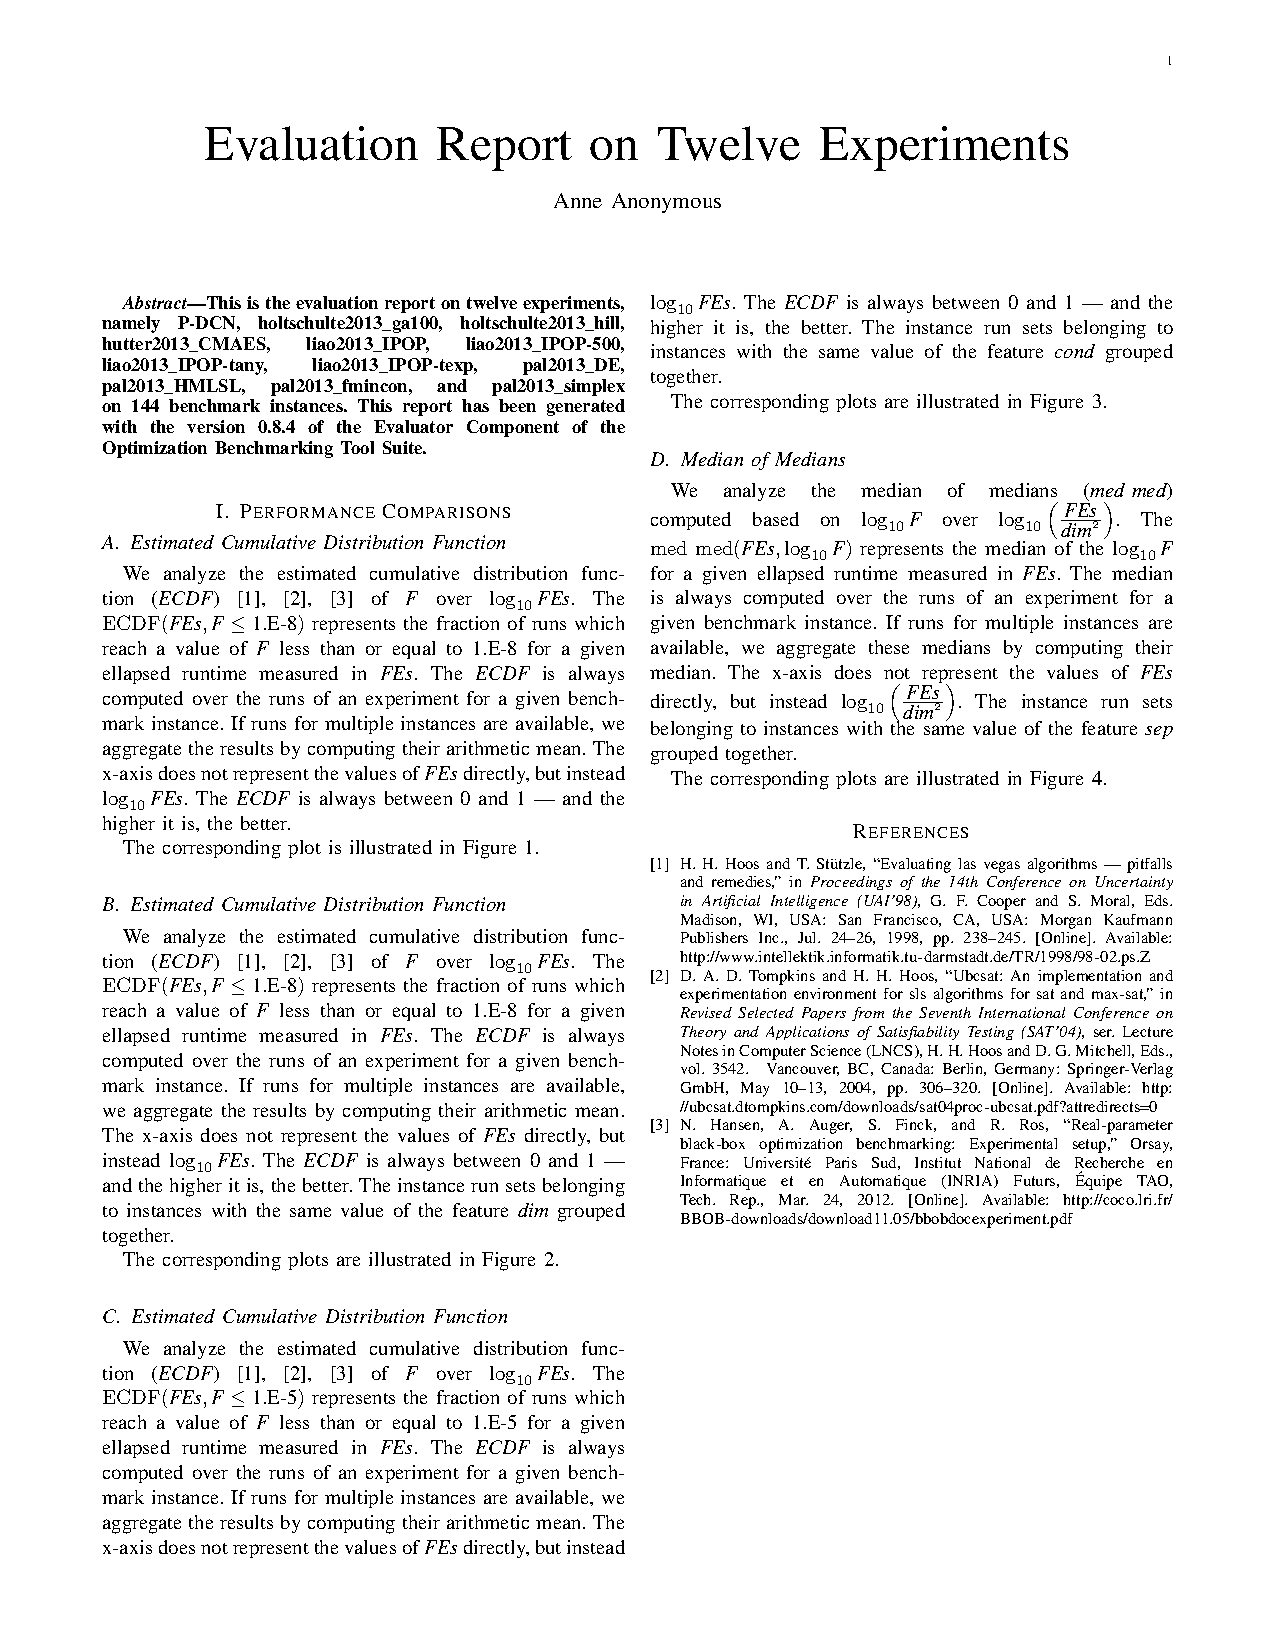
\includegraphics[width=0.3125\paperwidth,page=1]{\sharedPath/graphics/optimization/bbob/bbob_example_evaluation/bbob_example_evaluation_reports/IEEEtran_report.pdf}%
}%
}{%
first page of the report in \LaTeX\ for \texttt{IEEEtran}%
}{0.6}{0.29}{0.325}%
%
\end{frame}%